\fontfamily{\sfdefault}\selectfont
% XCircuit output "filt_design.tex" for LaTeX input from filt_design.ps
\def\putbox#1#2#3#4{\makebox[0.00000in][l]{\makebox[#1][l]{}\raisebox{\baselineskip}[0.00000in][0.00000in]{\raisebox{#2}[0.00000in][0.00000in]{\scalebox{#3}{#4}}}}}
\def\rightbox#1{\makebox[0.00000in][r]{#1}}
\def\centbox#1{\makebox[0.00000in]{#1}}
\def\topbox#1{\raisebox{-0.60\baselineskip}[0.00000in][0.00000in]{#1}}
\def\midbox#1{\raisebox{-0.20\baselineskip}[0.00000in][0.00000in]{#1}}
   \scalebox{1}{
   \normalsize
   \parbox{6.30000in}{
   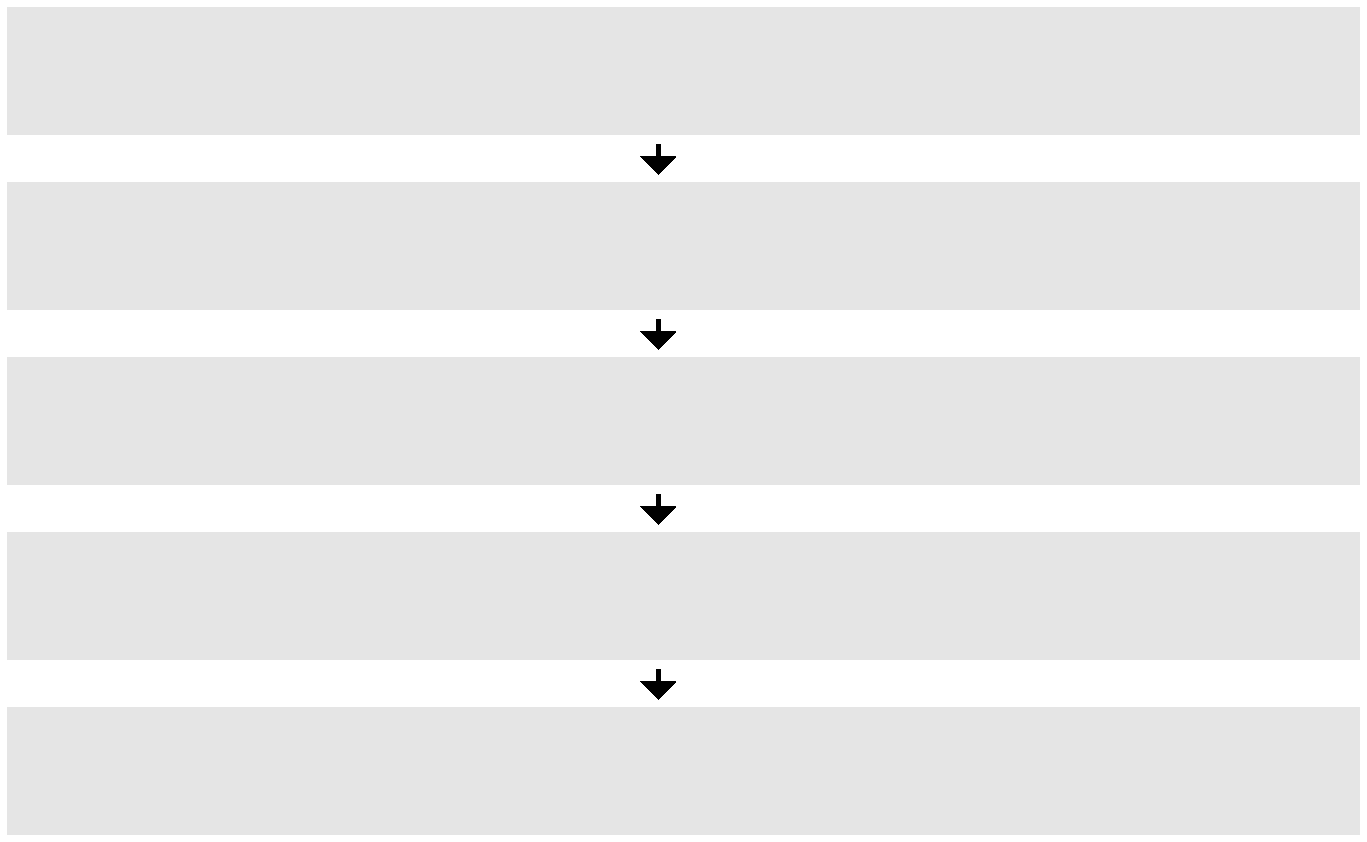
\includegraphics[scale=0.70000]{./figs/filt_design.pdf}\\
   % translate x=192 y=896 scale 0.38
   \putbox{1.90400in}{2.66700in}{0.96}{$T_{opt}(s)=\underset{T(s)}{\argmin}\int_0^{f_h}\mathcal{L}(\Delta f|T(s))d\Delta f$}%
   \putbox{0.09800in}{2.89800in}{0.96}{\textbf{Optimize continuous PLL closed loop response $T(s)$ for minimum total integrated phase noise.}}%
   \putbox{0.09800in}{3.71700in}{0.96}{\textbf{Specify PLL system parameters.}}%
   \putbox{0.18200in}{3.39500in}{0.84}{Divider ratio}%
   \putbox{1.52600in}{3.54200in}{0.84}{TDC resolution}%
   \putbox{1.55400in}{3.39500in}{0.84}{KDCO}%
   \putbox{0.18200in}{3.54200in}{0.84}{Reference frequency}%
   \putbox{3.57000in}{3.54200in}{0.96}{$S_{\Phi n_{DCO}}(f)$}%
   \putbox{0.12600in}{2.07900in}{0.96}{\textbf{Convert $T_{opt}(s)$ into discretized loop filter design.}}%
   \putbox{0.21700in}{1.90400in}{0.84}{Convert $T_{opt}(s)$ to loop filter $H_{LF}(s)$ based on provided system specifications.}%
   \putbox{0.21700in}{1.75700in}{0.84}{Use s-to-z transformation to convert $H_{LF}(s)$ to the discrete time $H_{LF}(z)$.}%
   \putbox{0.12600in}{1.26700in}{0.96}{\textbf{Second order optimize loop filter digital implementation.}}%
   \putbox{0.21700in}{1.09200in}{0.84}{Convert $H_{LF}(z)$ to direct form I implementation of its difference equation.}%
   \putbox{0.21700in}{0.94500in}{0.84}{Optimize number of bits per word used in digital implementation for quantization noise and filter accuracy.}%
   \putbox{0.12600in}{0.44800in}{0.96}{\textbf{Verify design with simulation.}}%
   \putbox{0.21700in}{0.27300in}{0.84}{Utilize behavioral, discrete event simulator to capture non-linear and discrete time effects.}%
   \putbox{0.21700in}{0.12600in}{0.84}{Monte-Carlo sampling for KDCO. initial frequency error to analyze stability, phase noise and lock time across PVT.}%
   \putbox{2.57600in}{3.54200in}{0.84}{DCO phase noise - }%
   } % close 'parbox'
   } % close 'scalebox'
   \vspace{-\baselineskip} % this is not necessary, but looks better
\fontfamily{\rmdefault}\selectfont
